\chapter{Conclusion}
\label{chapter:concl}

\begin{wrapfigure}{r}{60mm}
  \centering
  \vspace{-27em}
  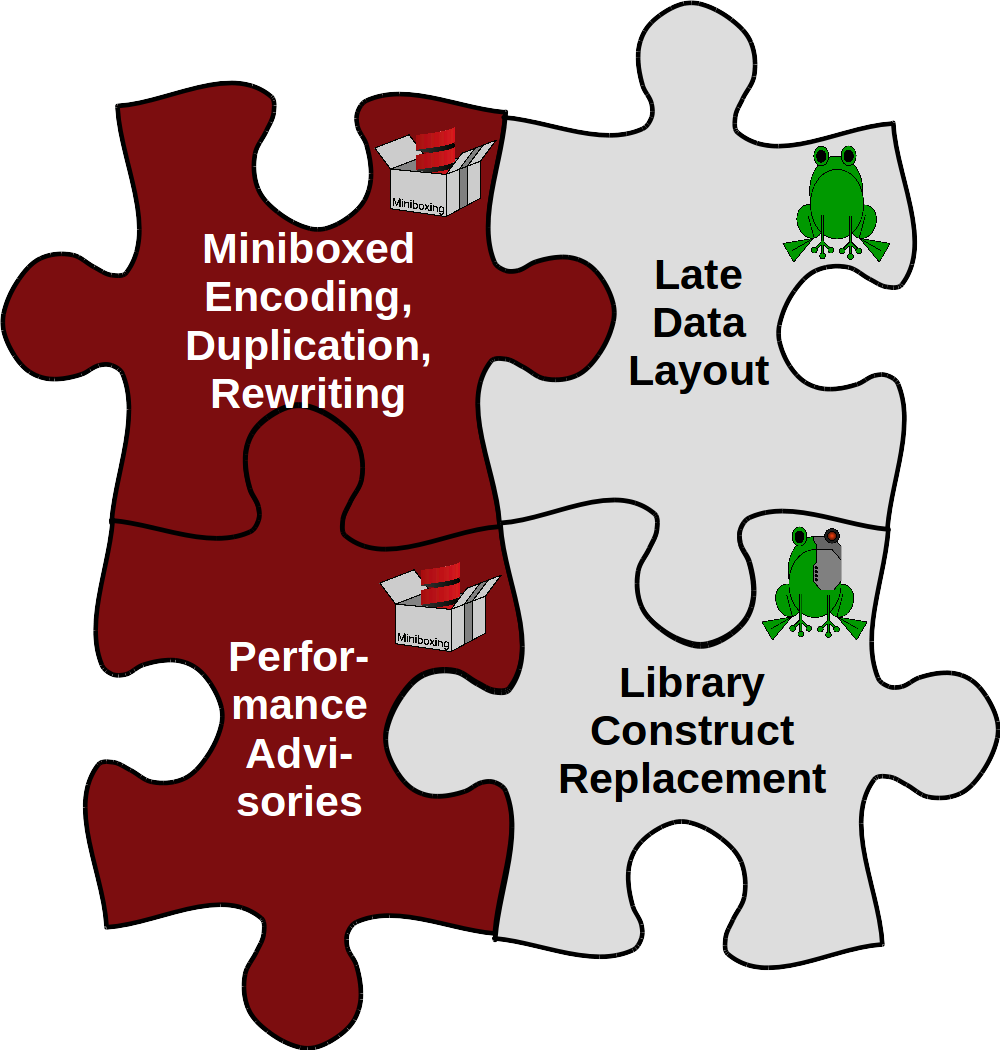
\includegraphics[width=60mm]{puzzle.pdf}
  \vspace{-30em}
\end{wrapfigure}

% The main artifact is miniboxing, but implementing it took more research than expected
The miniboxing transformation, which improves the interaction between generics and primitive types in the Scala programming language serves as the main motivation and technical artifact of the thesis. However, it took important side research to turn the idea of using long integers to store primitive types into a complete and reliable generics compilation scheme.

Late Data Layout grew out of the problem of scaling the code transformation in miniboxing to cover all abstract syntax tree patterns in the Scala compiler. Yet, it turned out to be a more general mechanism, supporting other important transformations as well.

The Data-Centric Metaprogramming approach started as transformation meant to integrate miniboxing with the functional aspects of Scala, but turned out to be a more general framework for programmers to express their own data representation transformations.

% Quickly recap: miniboxing, late data layout, data-centric metaprogramming and how this ties together
In retrospect, we're amazed at how many results came out of trying to solve a seemingly simple problem: reducing the amount of bytecode generated by specialization. Also, we are pleasantly surprised by the synergies between the different components that make up the miniboxing compilation scheme:

\begin{itemize}
  \item The miniboxed data encoding (top left tile) is more transparent and reliable when the transformation issues performance advisories (bottom left tile);
  \item Performance advisories (bottom left tile) are toothless compiler warnings if they are not backed by the support for interoperating with specialization. This support, which handles functions, tuples, arrays and type classes shares the scoped nature with the Data-Centric Metaprogramming approach (bottom right tile);
  \item The Data-Centric Metaprogramming approach (bottom right tile), despite its very ambitious goals, only needs a slightly improved version of the Late Data Layout mechanism (top right tile) to perform the program transformation;
  \item Late Data Layout (top right tile) forms the backbone of the miniboxing transformation, transforming duplicated code to use the miniboxed data encoding (top left tile);
\end{itemize}

% Many components we did not talk about
%There are also components that we did not mention: miniboxing has interesting interactions with reflection, carrying its own reified types, with the mix-in composition \cite{scalable-component-abstractions}, and with the erasure transformation in the Scala backend. These are all different aspects that did not fit into the thesis, but are important elements of the transformation.

% Mention the two types of transformations
\newpage
In the introduction (Chapter \ref{chapter:intro}), we have seen the two very different types of data representation transformations:
\begin{itemize}
  \item[(1)] Using compatible, drop-in replacements (miniboxing);
  \item[(2)] Using incompatible replacements and introducing conversions where necessary\\(Late Data Layout and Data-Centric Metaprogramming).
\end{itemize}

% Essentially, miniboxing serves as a compatibility layer over ldl-based transformations
From this perspective, miniboxing fine-tunes the compatibility layer introduced by specialization, introducing an interface at the top of the hierarchy and proposing performance advisories, which make the compatibility layer transparent. Thus, miniboxing can be seen as a compatibility layer added on top of an incompatible transformation, from type parameters to long integers. Realizing this inspires future work in the area.

\section{Future Work}

% Miniboxing = compatibility veneer. Could we mix compatibility + data-centric metaprogramming
Since miniboxing proposes a compatibility layer over an incompatible transformation, an interesting research question is whether the miniboxing scheme could be used to allow Data-Centric Metaprogramming transformations  inside generics. Indeed, initial research by Dmitry Petrashko indicates this may be the case. Furthermore, such a result would allow separating miniboxing into its two fundamental components: the generics compatibility layer and the data representation transformation, achieved using Data-Centric Metaprogramming.

% Late Data Layout formalization
Regarding the Late Data Layout mechanism, it would be very useful to devise a complete formalization, proving the optimality of the coercion push-down property. In \cite{ldl-form} we provide a definition of the transformation starting from the simply typed lambda calculus with |Nat|, |Bool| and |Unit|. However, this initial work only defines the transformation but does not proceed further to proving its properties. Since the LDL mechanism acts as the backbone of miniboxing, value class inlining and unboxing primitive types in the Scala compile backend, a formal proof of its properties would be highly desirable.

\begin{figure}[h!]
  \centering
  \vspace{0.6em}
  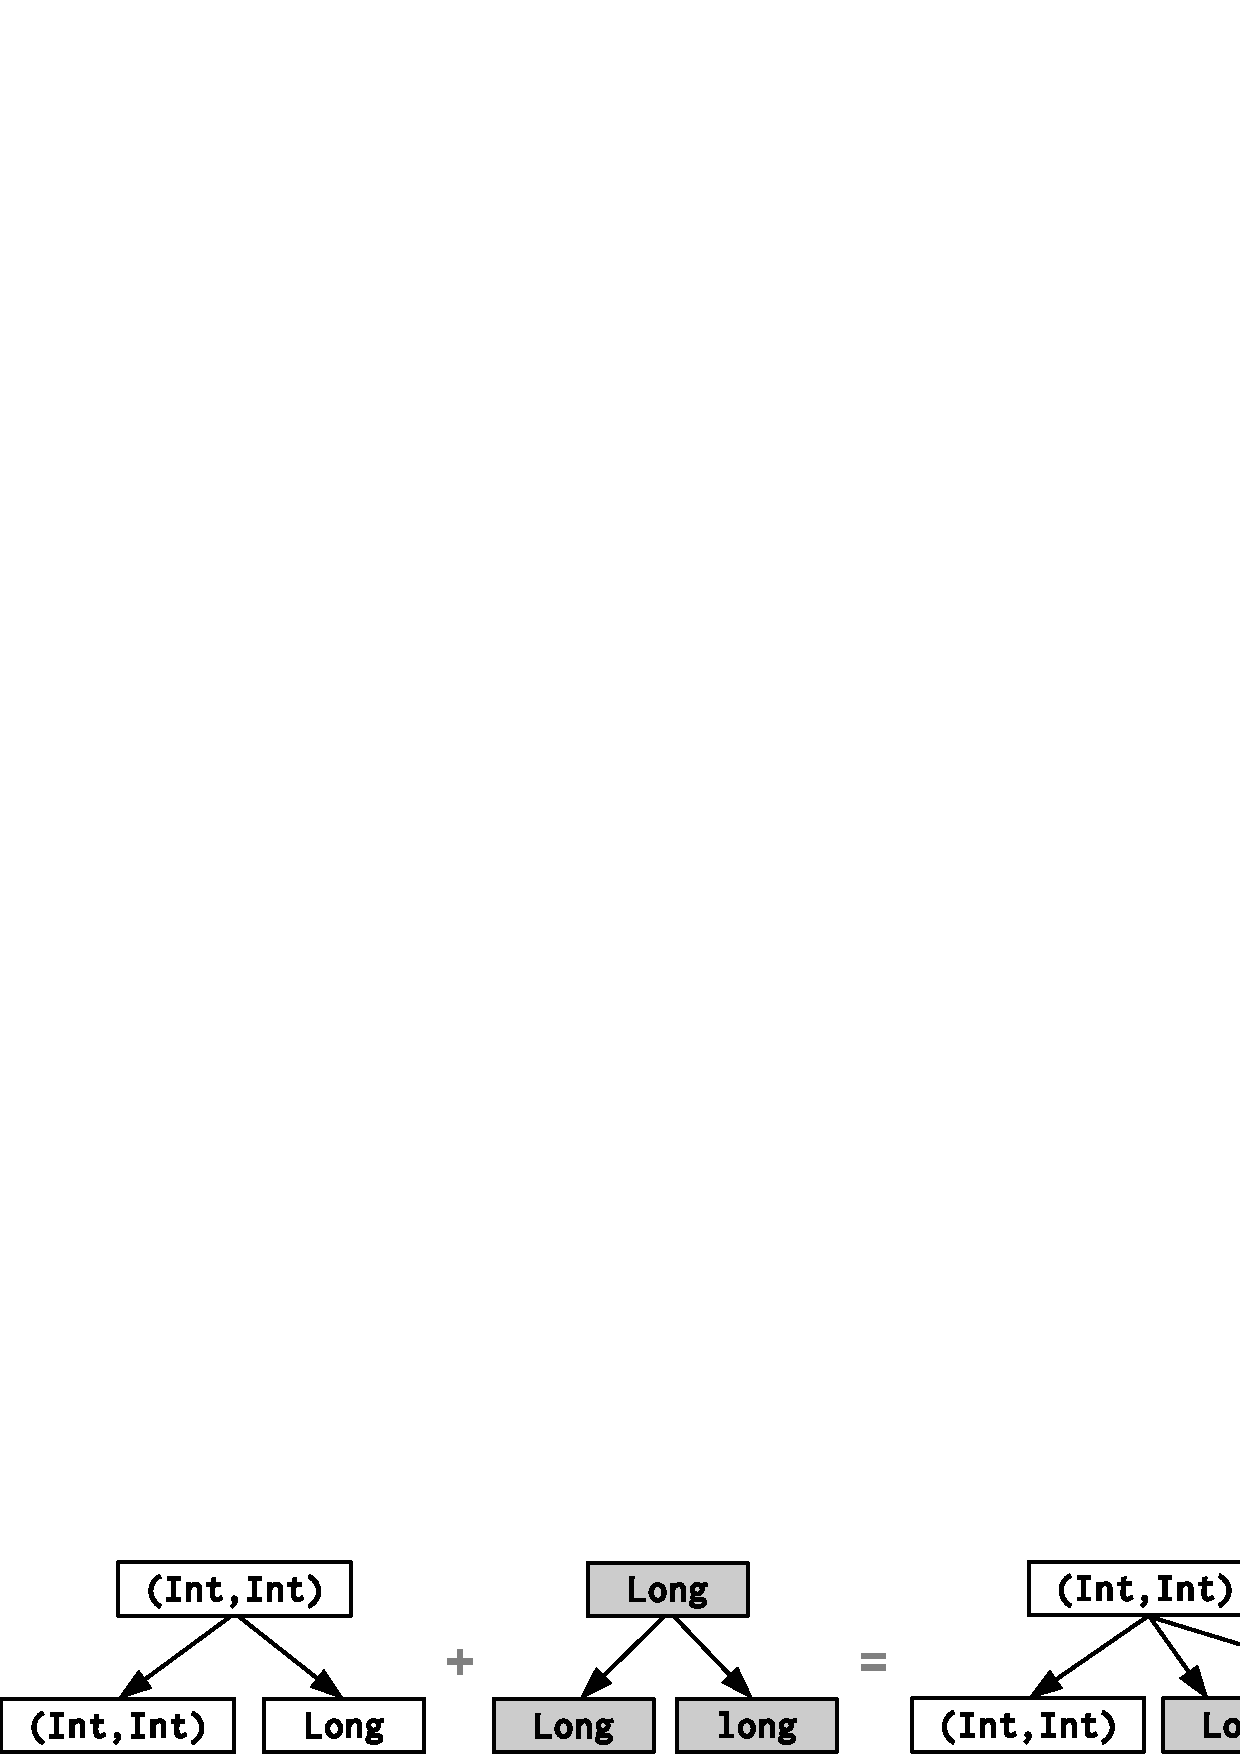
\includegraphics[width=0.8\textwidth]{ldl-combination.pdf}
  \caption{Late Data Layout transformation composition}
  \label{fig:ldl-composition}
  \vspace{-0.6em}
\end{figure}

% Composable transformations
Still within the realm of the Late Data Layout mechanism, an interesting question is what are the conditions that would allow several transformation steps to compose into one, as shown in Figure \ref{fig:ldl-composition}. And, even more interesting, in which cases the middle |Long| representation needs to be conserved? Answering these questions could open the door to more extensive data representation transformations, which are currently only accessible via manually-specified Data-Centric Metaprogramming description objects. Which brings us to the next topic.

% Static checks
One of the drawbacks of Data-Centric Metaprogramming is that programmers can break semantics by defining bypass methods whose code does not perform an equivalent operation.  An interesting direction would be to use symbolic execution to check the equivalence of the class method and the bypass method, eliminating semantics-changing transformations.

Another way to break program semantics is by defining a transformation that assumes the transformed scope is pure (i.e. does not have side effects), but to apply it to a scope that invalidates the constraints. To prevent such cases, it would be useful to allow transformation developers to express the constraints in the description objects and check whether each scope satisfies its corresponding constraints.


\section{Impact}

% Presented at 5 industrial conferences, many meetups
The data representation transformations in this thesis have been implemented as a Scala compiler plugins and have been documented on their respective websites \cite{miniboxing-www,ildl-www,ldl-www}. It has been presented at several developer conferences:

\begin{itemize}
  \item Spark Summit Europe 2015, Amsterdam, The Netherlands
  \item PNWScala 2014, Portland, OR, United States
  \item ScalaDays 2014, Berlin, Germany and 2015, San Francisco, CA, United States
  \item Devoxx UK 2015, London, United Kingdom
\end{itemize}

% Design of the Java performance extensions in the JVM
The miniboxing transformation will be part of the new incarnation of the Scala compiler (code name dotty). Furthermore, with the recent work on OpenJDK performance extensions (Project Valhalla\cite{goetz-specialization,valhalla-model2-announcement,valhalla-model2-implementation}), which include specialization and value class inlining, there has been an ongoing communication between our team and the Oracle architects designing Valhalla.

In all, the miniboxing plugin has 1110 commits from 9 contributors (other than the author) to which we are very grateful.

\section{Lessons Learned}

There are three lessons we derived from this thesis and hope others can use as well:

% Solving real problems
\textbf{Solve real problems then turn the solutions into research.} This is a suggestion given by Matei Zaharia, the creator of Spark, during a visit to EPFL in 2013. What the author subjectively understood is that the first step towards good research is focusing on a real problem and solving it. Then, research stems from analyzing the tradeoffs offered by the solution, whether it can be generalized and what are the other design choices possible. The work described in this thesis started the real problem of scaling specialization by reducing the amount of bytecode generated. And, indeed, solving this problem produced an avalanche of interesting research questions, which ultimately led to this thesis.

\textbf{Digging deeper uncovers more insights.} Once a problem has been solved, a natural question is how to transform it into research. Fortunately digging deeper, asking questions like ``Why is it so?'' and looking for synergies between different approaches can reveal non-obvious insights, which can later form the basis of research contributions. Late Data Layout stemmed from an intuition that other problems may be solved with the same approach as well, so the questions asked were: ``What other problems?'' and ``Why?''.

% Productizing
\textbf{Productizing research.} This is a lesson learned from the ``PhD Grind'' book of Philip Guo: it is not enough to come up with a good idea and publish it -- the idea should be tested in the real world, as a product. The miniboxing transformation was developed with this in mind, aiming for a product that developers can use in practice. Much of the energy has gone into stabilization, handling corner cases and generally the making the transformation useful. While some of the work was purely technical and did not lead to research questions, there were also many cases where a technical limitation led to asking questions that produced valid research contributions.
